\documentclass[UTF8]{ctexart}[a4paper,10pt]
\usepackage[thmmarks]{ntheorem}
\usepackage{amsmath}
\usepackage{amsfonts,amssymb} 
\usepackage{thmtools}
\usepackage[hmargin=2.5cm,vmargin=2.5cm]{geometry}
\usepackage{tikz-cd,tikz}
\usepackage{graphicx,float}
\usepackage{fancyhdr}
\usepackage{fourier-orns}
\usepackage{quiver}

%声明环境
\newtheorem{example}{例}[section]              
\newtheorem{algorithm}{算法}[subsection]
\newtheorem{theorem}{定理}[section]            
\newtheorem{definition}{定义}[section]
\newtheorem{axiom}{公理}[section]
\newtheorem{property}{性质}[section]
\newtheorem{proposition}{命题}[section]
\newtheorem{lemma}[theorem]{引理}
\newtheorem{corollary}[theorem]{推论}
{
    \theoremheaderfont{\sffamily}
    \newtheorem*{remark}{注解} 
}
\newtheorem{condition}{条件}
\newtheorem{conclusion}{结论}[section]
\newtheorem{assumption}{假设}
{
\theoremstyle{nonumberplain}
\theoremheaderfont{\bfseries}
\theorembodyfont{\normalfont}
\theoremsymbol{\mbox{$\Box$}}
\newtheorem{proof}{证明}
}
%定义命令
\def\N{\mathbb{N}}
\def\Z{\mathbb{Z}}
\def\Q{\mathbb{Q}}
\def\R{\mathbb{R}}
\def\C{\mathbb{C}}
\def\S{\mathbb{S}}
\def\D{\mathbb{D}}
\def\H{\mathbb{H}}
%外测度
\def\outmQ{m_*(Q)}

%页眉设计
\renewcommand 
\headrule{
\hrulefill
\raisebox{-2.1pt}
{\quad{\FourierOrns M T S N}\quad}
\hrulefill}
\pagestyle{fancy}

%超链接红色
\usepackage[colorlinks,linkcolor=red]{hyperref}

\usepackage{enumerate}


\title{Introduction to Dynamical System}
\author{颜成子游}
\begin{document}
\maketitle
\tableofcontents
\section{$S^1$上的扩张映射}
\begin{lemma}
    $f$是$S^1$上$C^1$扩张映射,$deg(f)=d$。$F$是$f$的提升.则$F:\R \to \R$是同胚,且$\forall y ,F^{-1}(y+d)=F^{-1}(y)+d$.
\end{lemma}
\begin{theorem}[Shub]
    $f,g$是$S^1$上的$C^1$扩张映射,且$deg(f)=deg(g)\neq 0$。则$f \sim g$.
\end{theorem}
\begin{proof}
    要找一个$h$是$S^1$上的同胚,使得$h \circ f=g \circ h$。在$S^1$上考虑并不方便,我们考虑提升。

    设$F,G$是$f,g$的提升。想找$H$是$h$的提升,使得:
    $$
    H \circ F=G \circ H
    $$
    即我们要研究方程:
    $$
    H=G^{-1}\circ H \circ F
    $$
    考虑压缩映像原理,我们记$T(H)=G^{-1}\circ H \circ F$。

    给出完备度量空间:$D=\{H \in C^0(\R,\R)|H(x+1)-H(x)=1\}$.定义距离为$d(H,J)=\sup_{x \in \R}|H(x)-J(x)|$.距离的定义合理性是显然的。

    容易验证$(D,d)$是完备度量空间。只需要给出逐点收敛的极限函数即可。

    考虑映射$T$:$G^{-1}\circ H \circ F(x+1)=G^{-1}\circ H (F(x)+d)=G^{-1}(H \circ F(x)+d)=G^{-1}\circ H \circ F(x)+1$。从而$T$是$D$上的映射。另一方面,记$\lambda=\inf_{x \in \R}|G'(x)|>1$,从而其逆映射的导数$|{G^{-1}}'(x)|<1$。计算:
    $$
    d(T(H),T(J))=\sup_{x \in \R}|T(H)(x)-T(J)(x)|
    $$
    由于$G^{-1}$的导数绝对值小于$1$,从而上式小于$d(H,J)$。(拉格朗日中值定理)。

    从而压缩映像的条件符合,存在唯一解$H_0$是不动点:$H_0 \circ F=G \circ H_0$。

    易知存在$h_0$:$h_0(e^{2\pi ix})=e^{2\pi i H_0(x)}$。这是$S^1$上一个映射度为1的$h_0$。目前我们需要证明$h_0$是同胚。

    先证明$H_0$是同胚。
    
    同理可证,存在唯一$\hat{H_0}$:$\hat{H_0} \circ G=F \circ \hat{H_0}$。从而:
    $$
    H_0 \circ \hat{H_0}\circ G=H_0 \circ F \circ \hat{H_0}=G \circ H_0 \circ \hat{H_0}
    $$
    因为方程:$G \circ H=H\circ G$有解$id$,且方程有唯一解。从而上述等式表明:$H_0 \circ \hat{H_0}=id$。同理后,这意味着$H_0$是同胚。

    从而存在$h_0,\hat{h_0}$.满足:

    $E\circ H_0=h_0 \circ E$

    $E\circ \hat{H_0}=\hat{h_0} \circ E$

    从而:
    $$
    (\hat(h_0)\circ h_0)\circ E=\hat{h_0}\circ E \circ H_0=E
    $$
    这意味着$(\hat(h_0)\circ h_0)$在$E$的像$S^1$上是$id$。同理后,$h$是同胚。

    最后验证$h,g,f$的关系:
    $$
    E \circ H_0 \circ F=h_0\circ E \circ F =h_0\circ f\circ E
    $$
    $$
    E \circ G \circ H_0=g \circ E \circ H_0 =g\circ h_0 \circ E
    $$
    从而在$S^1$上关系成立。
\end{proof}
\begin{corollary}
    $f$是$C^1$扩张映射,则$f$是$C^1$结构稳定的。
\end{corollary}

现在考虑一个模型:$f_\lambda(x)=\lambda x(1-x)$。考虑$\Lambda=\{x|\forall n,f^n(x)\in [0,1]\}$。

首先,$f(\Lambda)=\Lambda$。

其次,可以证明其是一个Cantor集合。

这个系统并不容易研究,但如果我们能够转化其为一个拓扑共轭的一个好研究的系统呢?
\section{符号动力系统}
\subsection{基本概念}
符号集合:$X=\{0,1,2,\dots,k-1\}$。

符号空间:$\Sigma_k=\prod_{i=0}^\infty X=\{(a_0a_1\dots)|a_i \in X\}$

定义符号空间之间的距离:$d(a,b)=\sum_{i=0}^\infty \dfrac{|a_i-b_i|}{(100k)^i}$

性质:

$\forall \epsilon >0,\exists N$使$\forall a,b \in \Sigma_k$:
$$
d(a,b)<\epsilon \Leftrightarrow a_i=b_i, i=0,1,2,\dots,N
$$

记$\alpha \in X$,记$[\alpha]=\{a\in \Sigma|a_o=\alpha\}$。可以证明$[0],[1],\dots,[k-1]$都是开集,闭集。说明整个空间是不连通的。

现在建立空间上的映射使之成为动力系统。

定义左移位映射$\sigma:\Sigma_k \to \Sigma_k$,$a_0a_1a_2\dots \mapsto a_1a_2\dots$,这是一个连续映射!

于是我们给出定义:单边符号系统$(\Sigma_k,\sigma)$。

我们断言以下性质:

1.$\overline{Per(\sigma)}=\Sigma_k$

2.$(\Sigma_k,\sigma)$是传递的:$\exists a\in \Sigma_k$使得$\overline{O(a)}=\Sigma_k$。

为了说明2,我们只需要让$a$中包含所有的组合。即$a$一个一个把所有的任意$n$组合全部举完。这样$a$迭代后总能与$\Sigma_k$中的每个元素任意近。

2还有一个说法:任意开集$U,V$非空,存在$n>0$,使得$f^n(U) \cap V \neq \emptyset$。
\subsection{回到刚才的问题——虫口模型}
回到刚才的单边系统$f_\lambda:\Lambda \to \Lambda$。
$f_\lambda(x)=\lambda x(1-x)$。

由于刚才我们说$\Lambda$是Cantor集合,因此$\Lambda$里的点可以被编码,具体写为:
$$
h:\Lambda \to \Sigma_2,x \mapsto a=(a_0a_1\dots)
$$

使得$f^nx \in I_{a_n}, \forall n \geq 0$。

其中$I_0$,$I_1$是使得$f(x)\in [0,1]$的两个分开区间。

显然:
$$
h \circ f=\sigma \circ h
$$
\begin{proposition}
$h$是同胚,从而有$(\Lambda,f) \thicksim (\Sigma_2,\sigma)$。 
\end{proposition}
\begin{proof}
先证明$h$是双射。$h$单射:设$x \neq y$但$h(x)=h(y)$。若$x,y$同属$I_0$或$I_1$,则$|f(x)-f(y)| \geq \mu |x-y|$。这意味着$|f^n(x)-f^n(y)|\geq \mu^n |x-y| \to +\infty$,矛盾!因为$|f^n(x)-f^n(y)|$总是一致有界的。

$h$满射:取$a=(a_0a_1a_2\dots)$,则要使得$h(x)=a$,则:
$$
x \in I_{a_0} \cap f^{-1}I_{a_1} \cap f^{-2}I_{a_2}\dots
$$
根据闭区间套$\{\bigcap_{n=0}^N f^{-n}I_{a_n}\}_{N=1}^\infty$,$x$存在。(为什么这些区间没有空集?)

再说明$h$和$h^{-1}$是连续的。

$h$连续:由于$|f'(x)|$有上界$\beta$,则$|f^n(x)-f^n(y)|\leq \beta^n |x-y|$。只要$x$,$y$足够小,那么他们在前$m$步处于同一个$I_i$。任取$\epsilon>0$,要使得$d(h(x),h(y))<\epsilon$,只需要前$N$步$x$,$y$处于同一个$I_i$。这一点已经可以实现了,只要$x,y$距离足够小。

$h^{-1}$连续:$\forall \epsilon>0$,$\exists N>0,\mu^N \epsilon >1$。 存在$\delta>0$,使得$d(a,b)<\delta \Leftrightarrow a_i=b_i,i=0,1,\dots,N$。记$h^{-1}(a)=x,h^{-1}(b)=y$,则$f^{i}(x),f^{i}(y)$同属$I_0$或$I_1$,$i=1,2\dots,N$。$1\geq |f^N(x)-f^N(y)| \geq \mu^N |x-y|$,从而$|x-y| \leq 1/\mu^N \leq \epsilon$。
\end{proof}
\begin{corollary}
    虫口模型是结构稳定的,因为稍稍扰动并不改变其与$(\Sigma_2,\sigma)$拓扑共轭的性质。
\end{corollary}
\subsection{Smale马蹄}
对区域$[0,1]\times [0,1]$,定义如下图的微分同胚$f$:
\begin{figure}[htbp]
    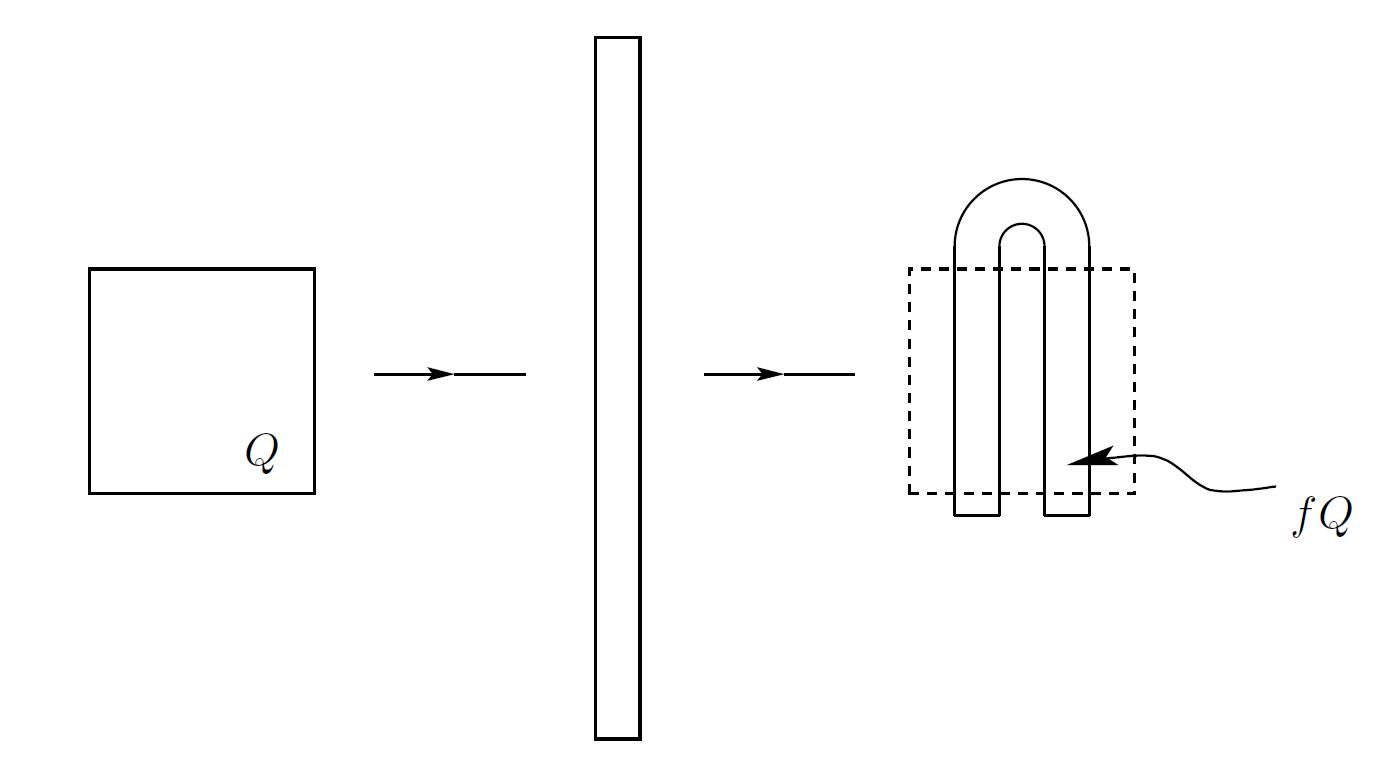
\includegraphics[scale=0.4]{Smale.jpg}
    \centering
\end{figure}

但为了研究动力系统,我们需要研究只在$Q$里面的变化:

\begin{figure}[htbp]
    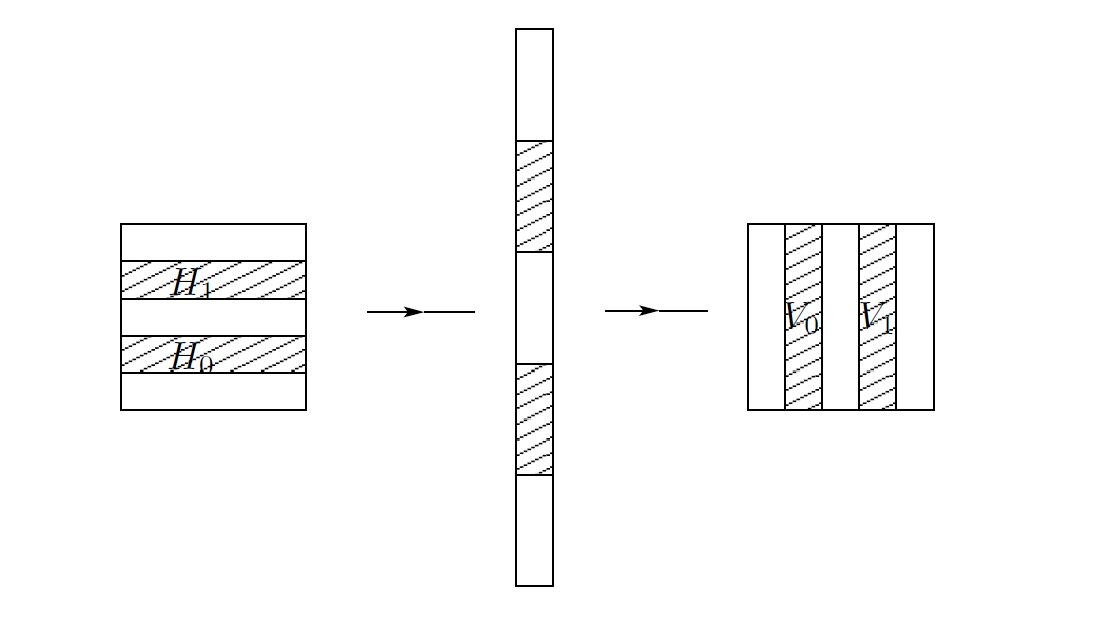
\includegraphics[scale=0.4]{Smalelimit.jpg}
    \centering
\end{figure}
\subsection{$T^2$上的扩张映射}
考虑$T^2=S^1\times S^1$,则可以定义$E:$
$$
E:\R^2 \to T^2 ,(x,y)\mapsto (e^{2\pi i x},e^{2\pi i y})
$$
此时$T^2$上的自同胚$f$可以诱导$\R^2$上的同胚$A$:
\begin{figure}[htbp]
    \centering
   \begin{tikzcd}
	{\R^2} && {\R^2} \\
	\\
	{T^2} && {T^2}
	\arrow["E", from=1-1, to=3-1]
	\arrow["f", from=3-1, to=3-3]
	\arrow["E"', from=1-3, to=3-3]
	\arrow["A"', from=1-1, to=1-3]
\end{tikzcd} 
\end{figure}
\begin{theorem}
    $f:T^2$是$C^1$结构稳定的。
\end{theorem}

\begin{definition}
    $f,g \in C^r(T^2)$。称$f,gC^r$近,若存在适当的提升使得$|Q-G|_{C^r}<<1$
\end{definition}

\begin{lemma}
    若$q,g$是$C^{0}-1/2$近的,且$Q,G$是提升。则$Q,G$对两个变量都是$1$-周期的。
\end{lemma}
为了证明引理,考虑$P_r=\{\varphi\in C^r(\R^2,\R^2)|\varphi \text{double per}\}$。从而我们可以再给出引理:
\begin{lemma}
    若$\varphi\in P_1$,且$|\varphi| <<1$,则$A+\varphi$可逆且$(A+\varphi)^{-1}=A^{-1}+\omega$,$\omega\in P_0$.
\end{lemma}
\begin{proof}
    首先说明是单射。当$\varphi$的模长足够小,由于$Ax=0$意味着$x=0$。

    为了说明其可逆,我们解方程:
    $$
    (A+\varphi)(A^{-1}+\omega)=id
    $$
    可以解出:
    $$
    \omega=-A^{-1}\varphi (A^{-1}+\omega)
    $$
    可以使用压缩映像原理来解决该问题。
\end{proof}
现在证明定理。
\begin{proof}
    设$A$是$f$的提升,$g$,$f$是$C^1$足够近,$G$是$g$的提升。令$G-A=\varphi \in P_1$.

    我们解方程:
    $$
    (id+\eta)(A+\phi)=(A+\varphi)(id+\eta)
    $$
    且
    $$
    \eta\in P_0
    $$
    $$
    \eta(A+\phi)=A\eta+\varphi (id+\eta)-\phi
    $$
    由于$A$在不同方向上有扩张,也有压缩。所以在一维上分别研究:
    
    设$A$的特征子空间为$E_1,E_2$,对应$\lambda_1<1,\lambda_2>1$。记$p$的投影为$p_i=\pi\circ p$。

    从而得到:
    $$
    \eta_1=(\lambda_1\eta_1+\varphi_1(id+\eta)-\phi_1)(A^{-1}+\omega)
    $$
    $$
    \eta_2=\frac{1}{\lambda_2}(\eta_2(A+\phi)-\varphi_2(id+\eta)+\phi_2)
    $$
    为运用压缩映像原理,定义:
    $$
    T_1\eta_1=(\lambda_1\eta_1+\varphi_1(id+\eta)-\phi_1)(A^{-1}+\omega)
    $$
    $$
    T_2\eta_2=\frac{1}{\lambda_2}(\eta_2(A+\phi)-\varphi_2(id+\eta)+\phi_2)
    $$
    从而定义$T:P_0 \to C^0(\R^2,\R^2),\eta=\eta_1+\eta_2 \mapsto T_1(\eta_1)+T_2(\eta_2)$。

    要验证以下事实:
    \begin{enumerate}
        \item $\forall \eta \in P_0,T(\eta)\in P_0$
        \item $\forall \eta\in P_0$,令$|\eta|=\max(|\eta_1|,|\eta_2|)$.这是一个完备度量。
    \end{enumerate}
    然后也是一个压缩映射:
    $$
    \eta,p \in P_0,|T\eta-Tp|<|\eta-p|
    $$
    验证压缩映像需要验证114514次(悲)
\end{proof}
\section{混沌}
一种混沌:$0<d(x,y)\lll 1$,总存在$n>0$,$d(f^n(x),f^n(y))>\epsilon_0$

混沌描述的是一种初值敏感依赖。因为初值的观测总是有误差的,如果系统混沌,那么系统难以进行长期的预测。

\subsection{混沌的定义}
\begin{definition}[Li-Yorke混沌]
    $0<d(x,y)\lll 1$,总存在$n>0$,$d(f^n(x),f^n(y))>\epsilon_0$
\end{definition}
这种混沌有定理:
\begin{theorem}
    $f:[0,1]$连续。若$f$有3-周期点,则对$\forall n>0$,有$n$周期点。
\end{theorem}
\begin{theorem}[Sharkovsky定理]
    把自然数排列:先排列奇数:$3,5,7,9\dots$,再排列$2\times 3,2\times 5,\dots,4\times 3,4\times 5,\dots,2^k\times 3,2^k \times 5,\dots,2^{k+1},2^k,\dots,8,4,2,1$.

    若$f:[0,1]$有$p$周期点,则任何在$p$后的$q$,$f$都有$q$周期点。
\end{theorem}
\end{document}